\chapter{引言}
\section{研究背景与意义}
建筑运行能耗长期居高不下。国际能源署在《Energy Efficiency 2023》中指出，建筑运行用能约占全球终端用能的三分之一，其中暖通空调与生活热水占据主要份额\cite{iea2023}。单栋建筑的节能控制相对简单，通过主机调节与定时策略即可取得成效；然而对于由多栋异构建筑组成的社区，问题显著复杂化：暖通、热水储能、电池与光伏等多种设备相互耦合，共用同一配电馈线、同一套分时电价与碳强度曲线。若A楼在高电价时段放电而B楼恰好在充电，社区总峰值反而可能被推高。这种耦合特性决定了建筑群控制并非单机回路的简单叠加，而是一个多智能体、多目标、部分可观测的序贯决策问题。

实际工程中的矛盾主要集中在四个方面。第一，经济性目标要求将负荷转移至电价低谷时段，而电网友好目标要求削峰并抑制爬坡，二者的最优工作点往往相互错开；第二，低碳运行希望在光伏大发、碳强度较低的时段多用电，这与实时电价的引导方向并不总是一致；第三，设备利用率与室内舒适度之间存在固有权衡，设备多运行一分、室温多偏离一分，效率与舒适便开始冲突；第四，中央协调器虽在理论上可获取全局信息，但现场通信、隐私与计算延迟等约束使完全集中式决策难以实现。因此，难点不仅在于寻得一个低能耗动作，更在于不确定性、异构性与安全约束并存的条件下，给出一个可解释、可落地的折中方案。

工程实践中应用最广泛的仍是规则控制（Rule-Based Control, RBC）与PID控制。基于运维经验的规则直观可靠、部署迅速，但参数一经固定，便难以适应次日电价走势与碳强度变化。模型预测控制（MPC）将约束写入滚动优化，控制效果良好\cite{mps2018,drgona2020mpc}；然而一旦模型失准，或建筑数量增多、设备类型复杂化，混合整数规划的求解规模迅速上升，在线运行面临较大计算压力。开题阶段梳理的BOPTEST框架为这类策略提供了高保真仿真与标准化测试用例，并以容器化部署和RESTful API支持MPC等先进策略的快速部署与评估\cite{boptest2021}；但其依赖精确模型、部署成本较高的特点意味着并非所有楼宇模型均可直接套用，这正是后文将MARL封装为易用闭环平台的动因之一。

强化学习提供了另一条技术路线：不依赖完整机理模型，通过与环境交互试错来获取长期回报。DQN将值函数引入神经网络\cite{mnih2015}，DDPG与SAC处理连续动作空间\cite{ddpg2016,haarnoja2018}，PPO利用裁剪机制稳定更新步长\cite{ppo2017}。将每栋建筑视为一个智能体，问题即转化为多智能体强化学习（MARL）\cite{marl2021}。该路线保留了分布式执行的可扩展性，又能通过集中式评论家或共享意图刻画建筑间的耦合关系，LSD-MADDPG甚至仅共享离散化意图以兼顾隐私\cite{wilk2024}。然而纯MARL亦存在明显局限：收敛需要大量交互样本，环境非平稳性使训练过程波动，随机探索可能触及设备或舒适度边界，在分布外场景下性能亦容易下降\cite{citylearn2020,citylearn2024}。

CityLearn的出现，很大程度上是为了解决评估标准不统一、算法难以公平比较的问题。2020年开源版本将多栋建筑的可调负荷、电池动作与社区总费用、峰值、爬坡、不适率等KPI统一绑定\cite{citylearn2020}；v2版本进一步补充了韧性、住户行为与碳感知机制\cite{citylearn2024}，项目主页持续维护数据与接口\cite{ielabcitylearn}，官网同步发布环境代码与文档入口\cite{citylearnnet2025}。四年的通用任务框架演进确立了``同一套任务比较不同算法''的范式\cite{nagy2025fouryears}，基于Gym环境的多目标控制基准进一步将成本、碳排放与电网负荷纳入同一度量体系\cite{nweye2024applications}。围绕该平台举办的Challenge将规则控制、预测优化与强化学习纳入同一任务进行评测\cite{citylearnchallenge2023,iclrenergy2023}，CORAIL等团队的系列工作也推动社区能源管理成为研究热点\cite{corail2024}。基于CityLearn开展区域需求侧管理的集中式柔性Actor-Critic早期尝试\cite{kathirgamanathan2020}，与离线多智能体数据集及基线研究\cite{formanek2023}，分别从集中学习与离线泛化两个侧面说明了统一基准的价值与小样本条件下的困难。

2023年Challenge冠军方案CHESCA（Community-based Hierarchical Energy Systems Coordination Algorithm）采用了不同的技术路线：中央—本地分层架构，结合电价感知规划、峰值管理、负荷跟踪与电池路径搜索实现控制\cite{chesca2024}。该方案无需大规模在线训练即可稳定运行，且具备良好的可解释性，在数据有限的现场尤其适用。其局限同样明确：规则参数与预测模型相对静态，面对设备老化、负荷漂移与极端天气时响应迟缓。CHESCA能够给出稳健的基准动作，但无法自主探索``在安全边界之内还能挖掘出多少多目标收益''。

残差强化学习恰好可以弥补这一不足。Johannink等在机器人任务中提出：策略不从零输出绝对动作，仅学习相对于基线的修正量\cite{residual2019}。基线保障安全性与样本效率，神经网络负责挖掘长期增益。将该思想迁移至多智能体建筑群场景，每栋建筑基于本地观测为自身基线动作施加小幅修正，训练端利用全局信息评估联合收益，即形成``先验保底、学习增益''的混合范式。住宅建筑多智能体能源管理\cite{marlresidential2019}、面向社区成本最小化的MARL与线性规划混合方法\cite{costmin2024community}、里尔大学2025年博士论文对智能社区能量管理的系统梳理\cite{lille2025thesis}，以及HVAC最优控制的早期对比研究\cite{chen2020hvac}、智能家居深度强化学习\cite{zhang2022ems}与建筑控制强化学习综述\cite{wang2021review}，均从不同侧面表明该混合路线值得深入研究。联邦多智能体DDPG将CTDE与隐私保护相结合\cite{fedmadDPG2024}，其所依赖的FedAvg\cite{mcmahan2017fedavg}与FedProx\cite{li2020fedprox}，亦为后续隐私敏感场景预留了技术接口。

本课题的价值可从两个层面分析。理论层面，``稳健规则基线+轻量残差MARL''为小样本、安全关键的多智能体决策提供了一个可复用的范式；工程层面，覆盖数据管理、算法配置、仿真任务、KPI计算与决策展示的可视化平台能够降低使用门槛，使能源管理者理解策略调整的原因及其带来的成本与碳排放收益，从而支撑绿色运行与需求侧管理的实际决策。

\section{国内外研究现状}
\subsection{国外研究现状}
国外相关研究大致经历了四个阶段：单设备定值控制、MPC优化、强化学习，以及社区级标准化测试。

早期研究以设备本体控制为主，采用回差控制、时间计划与焓值判据等方法，计算量小、可靠性高，但仅依赖局部反馈，无法实现日前负荷转移，也不具备多目标优化能力。MPC将建筑热动态建模，每个控制周期求解一次有限时域优化问题，在天气与价格预报准确时可显著降低成本；然而模型阶次选择、参数辨识、预报误差与求解器规模中任一环节出现问题，均会影响控制效果\cite{mps2018}。建筑数量增多后，各建筑热容、设备容量与使用模式均不相同，集中式MPC面临计算瓶颈，分散式方案则需精心设计信息共享机制，否则将陷入个体最优而全局次优的局面\cite{drgona2020mpc}。

深度强化学习依靠与环境交互试错来学习长期回报最大化策略。在单建筑HVAC场景，Wei等采用深度强化学习调节温度设定值\cite{wei2017hvacdrl}，Mbuwir等利用批量强化学习管理微网电池\cite{mbuwir2017residential}，Moriyama等构建了电耗优化的强化学习测试平台\cite{nagy2018marlbuilding}；多建筑场景则将每栋建筑或每类设备建模为智能体，采用MADDPG、MAPPO、QMIX、独立SAC等算法\cite{lowe2017,rashid2018,yu2022mappo,haarnoja2018}，COMA利用反事实基线解决信用分配问题\cite{foerster2018counterfactual}。CityLearn论文将独立学习、CTDE与全集中策略进行系统比较，指出了核心矛盾：仅以个体成本为奖励时峰值容易叠加，需以标准化KPI引导算法设计\cite{citylearn2020}。v2版本与Challenge综述进一步确认：在数据稀缺、预算有限且安全要求较高的条件下，纯MARL的探索噪声与不稳定更新容易产生性能较差的控制动作\cite{citylearn2024,citylearnchallenge2023}。

CHESCA是2023年竞赛中具有代表性的混合解决方案\cite{chesca2024}。该方法将协调过程分解至多个时间尺度：日前电价感知规划、日内峰值与爬坡管理、本地负荷跟踪以及电池动作搜索。中央层依据社区总负荷向各建筑下发参考信号，本地层根据自身状态将指令落实到具体设备；电池调度采用综合考虑电价、峰值与爬坡代价的路径搜索方法安排充放电。该方案无需很长的历史数据即可稳定运行，多项KPI均具有竞争力。由于其结构清晰、可解释性强且易于部署，本文选择其作为基准方法。

残差控制是另一条可借鉴的技术路线。Johannink等提出的残差强化学习使策略从安全的初始策略出发进行学习，样本效率优势明显\cite{residual2019}。在能源系统场景中，残差幅度限制、动作掩码与安全投影需要协同设计，否则局部最优的小幅修正也可能导致社区峰值或舒适度指标恶化。

\subsection{国内研究现状}
近年来，国内建筑节能研究的重心逐步从设计节能转向运行节能，政策与标准先行引导。张贞等梳理了中国绿色建筑发展与建筑节能的形势与任务，指出绿色理念正融入规划与改造的全过程\cite{zhangzhen2024}；既有建筑改造强调在线监测、诊断与优化。综述类研究指出，MARL在电网调度与复杂系统控制中具有广阔前景，但非平稳性、信用分配与可扩展性仍是主要挑战\cite{marl2021,zou2020rlsurvey,wang2021magame}；胡裕靖从博弈、均衡与知识迁移角度对MARL理论的梳理\cite{huyujing2015}，至今仍是理解多智能体非平稳性与均衡问题的重要参考。方法层面，凌飞等提出PID-Lagrange-SAC复合深度强化学习调控策略，利用拉格朗日乘子约束抑制智能体行为越界\cite{lingfei2025}，与本文安全投影的设计动机一致；薛聚星研究了联邦强化学习框架下的智慧楼宇低碳运行方法，以隐私保护为前提实现多建筑协同\cite{xuejuxing2023}；丁俐夫将可观测性分析、收敛性证明与电力系统工程应用相结合，为高比例可再生能源电力系统的自治运行建立了规范\cite{dinglifu2023}；薄婉琳针对多区域建筑暖通空调系统提出了深度强化学习控制方法\cite{bowanlin2024}；刘健开发的建筑节能统计信息管理系统代表了管理侧信息化的早期形态\cite{liujian2020}。亦有研究从住户交互视角探讨主动节能与隐私协同问题\cite{occupant2024}。经典强化学习教材与综述对MDP、策略梯度与值函数方法进行了系统阐述\cite{sutton2018}，Gym\cite{openai_gym2016}与Gymnasium\cite{gymnasium2024}一脉相承的接口标准，则是CityLearn得以构建的技术基础。

当前研究的主要瓶颈在于数据。单建筑运行数据受隐私、产权与计量口径限制，难以公开；仿真数据又无法完全覆盖设备老化、人员行为随机性与环境偏差。采用CityLearn这类可复现、KPI完备、数据开放的平台，至少能够在公平基线上开展算法比较。工程落地层面，国内多数能源管理系统仍停留在数据采集、展示与阈值报警阶段，算法层相对薄弱；即使接入了MPC或强化学习算法，也普遍缺乏任务调度、模型版本管理、参数追踪与决策解释能力。将算法研究与可视化平台协同建设，是研究成果从论文指标走向运维实践的必要路径。

\subsection{研究现状总结与问题提出}
上述两条技术路线具有互补性，但长期未能有效结合：规则与规划类方法安全稳健、易于部署，但缺乏长期自适应能力；MARL能够处理复杂多目标问题，但在小样本条件下缺乏稳定性与约束保证。CHESCA证明了强基线的价值，但尚未引入残差学习能力；纯多智能体方法能够学习协同修正策略，独立运行时又缺乏鲁棒性。平台层面则普遍缺少实验管理、决策解释与工程复用能力。基于此，本文首先归纳改进前的核心难题，进而给出一一对应的解决方案，作为全文的研究总纲。总体关系如图\figref{核心难题与改进方案}所示。
\begin{figure}[htb]
    \centering
    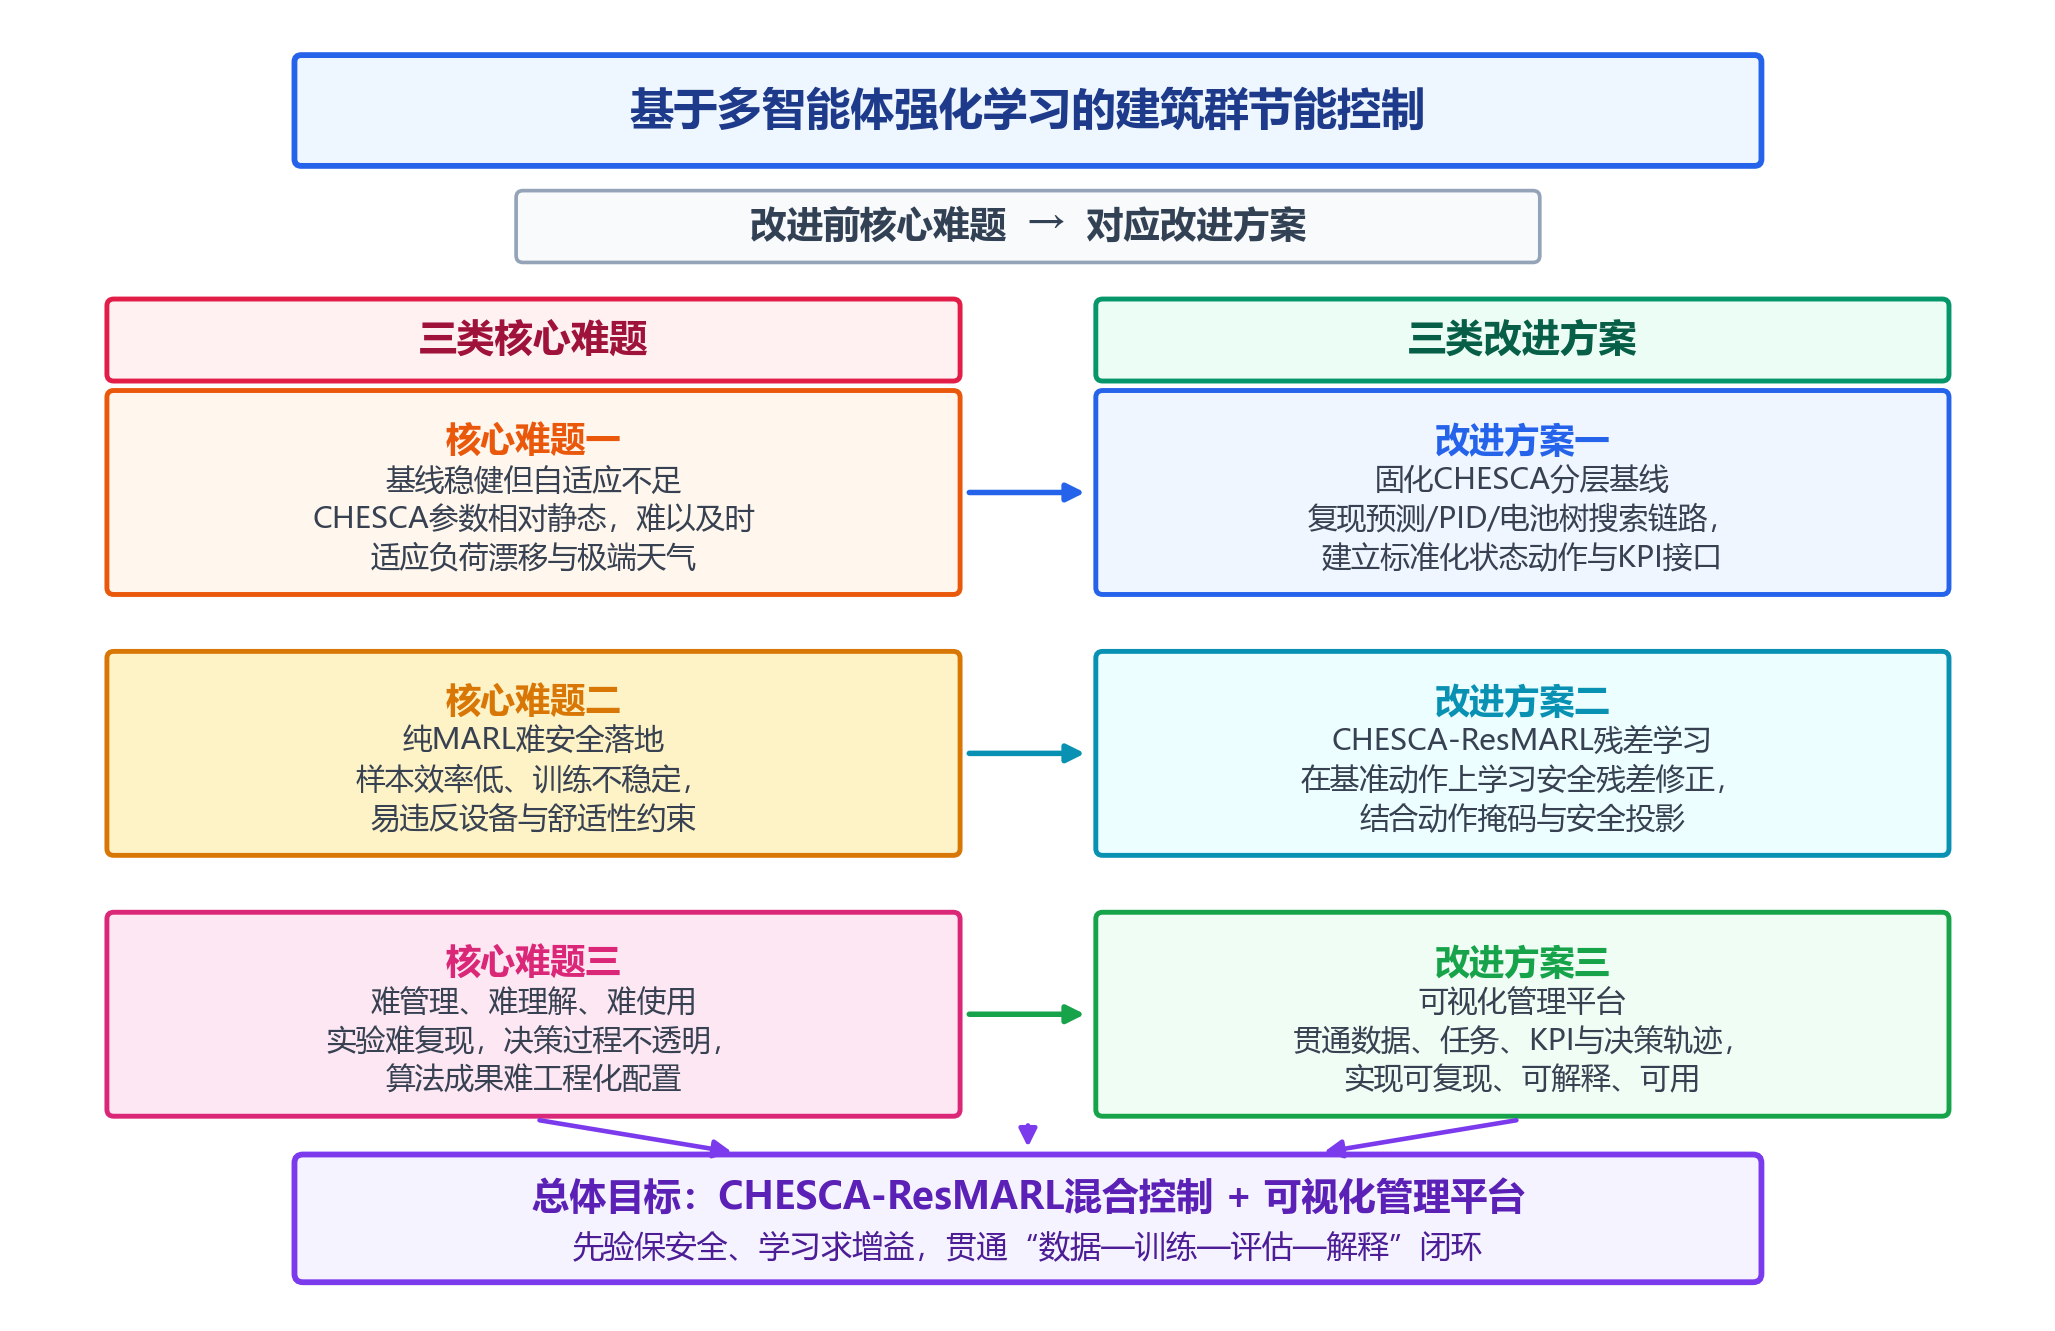
\includegraphics[width=0.92\textwidth]{./images/pictures/核心难题与改进方案.png}
    \centering\bicaption{核心难题与改进方案}{Core Challenges and Improvement Solutions}
    \label{核心难题与改进方案}
\end{figure}

\section{改进前的核心难题与改进方案}
\subsection{改进前的核心难题}
从竞赛算法到可复现、可解释、可部署的系统，本文识别出三类不可回避的核心难题。

（1）难题一：基线稳健但自适应能力不足。CHESCA依靠预测、规则与电池搜索给出了可解释的控制基准，在数据有限的条件下亦能稳定运行。然而其PID增益、搜索权重与电价分位阈值相对固定，面对负荷漂移、设备老化、电价机制调整与极端天气时响应迟缓；当电价机制、设备特性与舒适度要求发生变化时，固定策略只能维持基本可用水平，无法充分挖掘安全边界内的潜在增益。

（2）难题二：纯学习方法性能潜力大但难以安全落地。将建筑建模为智能体后，长期协同策略确实可以通过学习获得，但在CityLearn这类连续动作、强耦合场景中，样本效率低、环境非平稳、信用分配困难与探索不安全等问题同时存在。随机探索可能越过SOC、功率或舒适度边界；在预算有限且缺乏安全层的条件下，纯MARL很难一次性达到工程可接受的稳定性与可复现性。

（3）难题三：实验管理分散、决策过程不透明、成果难以复用。单次实验同时产生配置快照、时序观测、动作轨迹与多维KPI。缺乏统一的数据管理、任务调度与归档机制时，实验复现无从谈起；仅提供最终KPI而不展示基线动作、残差修正与投影过程，运维人员无法理解``为何如此调节''；算法分散于各类脚本之中，非算法背景人员难以完成配置、比较与应用。

\subsection{对应的改进方案}
本文以CityLearn为仿真基准、CHESCA为工程基线，提出CHESCA-ResMARL混合控制策略并构建配套可视化平台。总体思路可以概括为：CHESCA保障动作的可行性与安全性，残差MARL在受限范围内进行策略修正，平台实现实验管理与决策解释的全程贯通。

（1）方案一：复现并固化CHESCA，建立标准化实验链路。梳理预测层、本地动作初稿、未来用电估计、社区电池树搜索与净负荷回写各环节；统一建筑与社区的状态、动作、约束与KPI接口，使NOCONTROL、纯CHESCA与混合策略能够在相同数据与指标体系下进行比较。该方案回应难题一，同时为残差学习提供可退化的安全锚点。

（2）方案二：CHESCA-ResMARL残差多智能体框架。在基准动作$a^{base}$基础上，各建筑智能体依据本地观测输出连续残差，以
\begin{equation}
a^{final}=\mathrm{clip}\big((1-\alpha)a^{base}+\alpha a^{RL}\big)
\end{equation}
或等价的$a^{base}+\alpha\Delta a$形式合成最终动作。利用残差系数$\alpha$、通道掩码（DHW/ELE/TMP）与安全投影将探索范围约束在边界之内；强化学习侧为每栋建筑独立的SAC策略，执行阶段仅依赖本地观测。该方案回应难题二，实现``先验保安全、学习求增益''的设计目标。

（3）方案三：算法—平台一体化的可视化管理。基于Vue、Spring Boot、MySQL与Python算法组件，覆盖权限管理、数据集管理、算法登记、参数配置、异步仿真、KPI图表、决策轨迹与日志归档等功能。以任务标识贯通配置、运行与结果数据，使研究者能够复现实验，管理者能够理解基线、残差与投影如何合成最终动作。该方案回应难题三。

本文的具体研究内容包括：问题建模、CHESCA复现、残差策略与多目标奖励设计及评价、平台研发。潜在贡献为：面向CityLearn场景的CHESCA-ResMARL分层残差框架；兼容规则规划、强化学习、任务调度与KPI分析的一体化接口；在可运行系统中贯通``数据—训练—评估—解释''完整链路。

\section{论文组织结构}
全文共分六章。第一章为引言，阐述建筑群节能控制的现实需求与理论难点，综述国内外研究现状，给出难题—方案总体框架；第二章介绍相关工作与技术，涵盖强化学习、平台技术、残差控制与CityLearn，并单设一节详细解析CHESCA三类动作生成技术与XGBoost预测方法；第三章进行系统需求与架构分析；第四章阐述系统构建与技术实现，单列前端系统功能介绍并预留界面截图位置；第五章给出实验与结果分析，包括Postman接口测试、日志分析与结果可视化；第六章为讨论与展望。
